\section{VDB Implementation}\label{vdb:sec}

This section covers the theory and implementation of the VDB data structure.

The VDB (Volumetric Dynamic B-tree) is an advanced data structure designed to efficiently and flexibly represent sparse volumetric data. It is organised hierarchically, consisting of root, internal, and leaf nodes, each serving distinct purposes within the structure. This section begins by explaining in detail how VDB is structured and continues by going through the implementation of the data structure in the rendering engine.

\subsection{Data Structure}
\label{vdb:ds}

VDBs are sparse, shallow trees with a fixed depth but expandable breadth capable of covering a virtually infinite spatial domain. This design enables the VDB to efficiently manage large and complex datasets by adjusting the level of detail dynamically and minimising memory usage.

\begin{figure}[H]
  \centering
  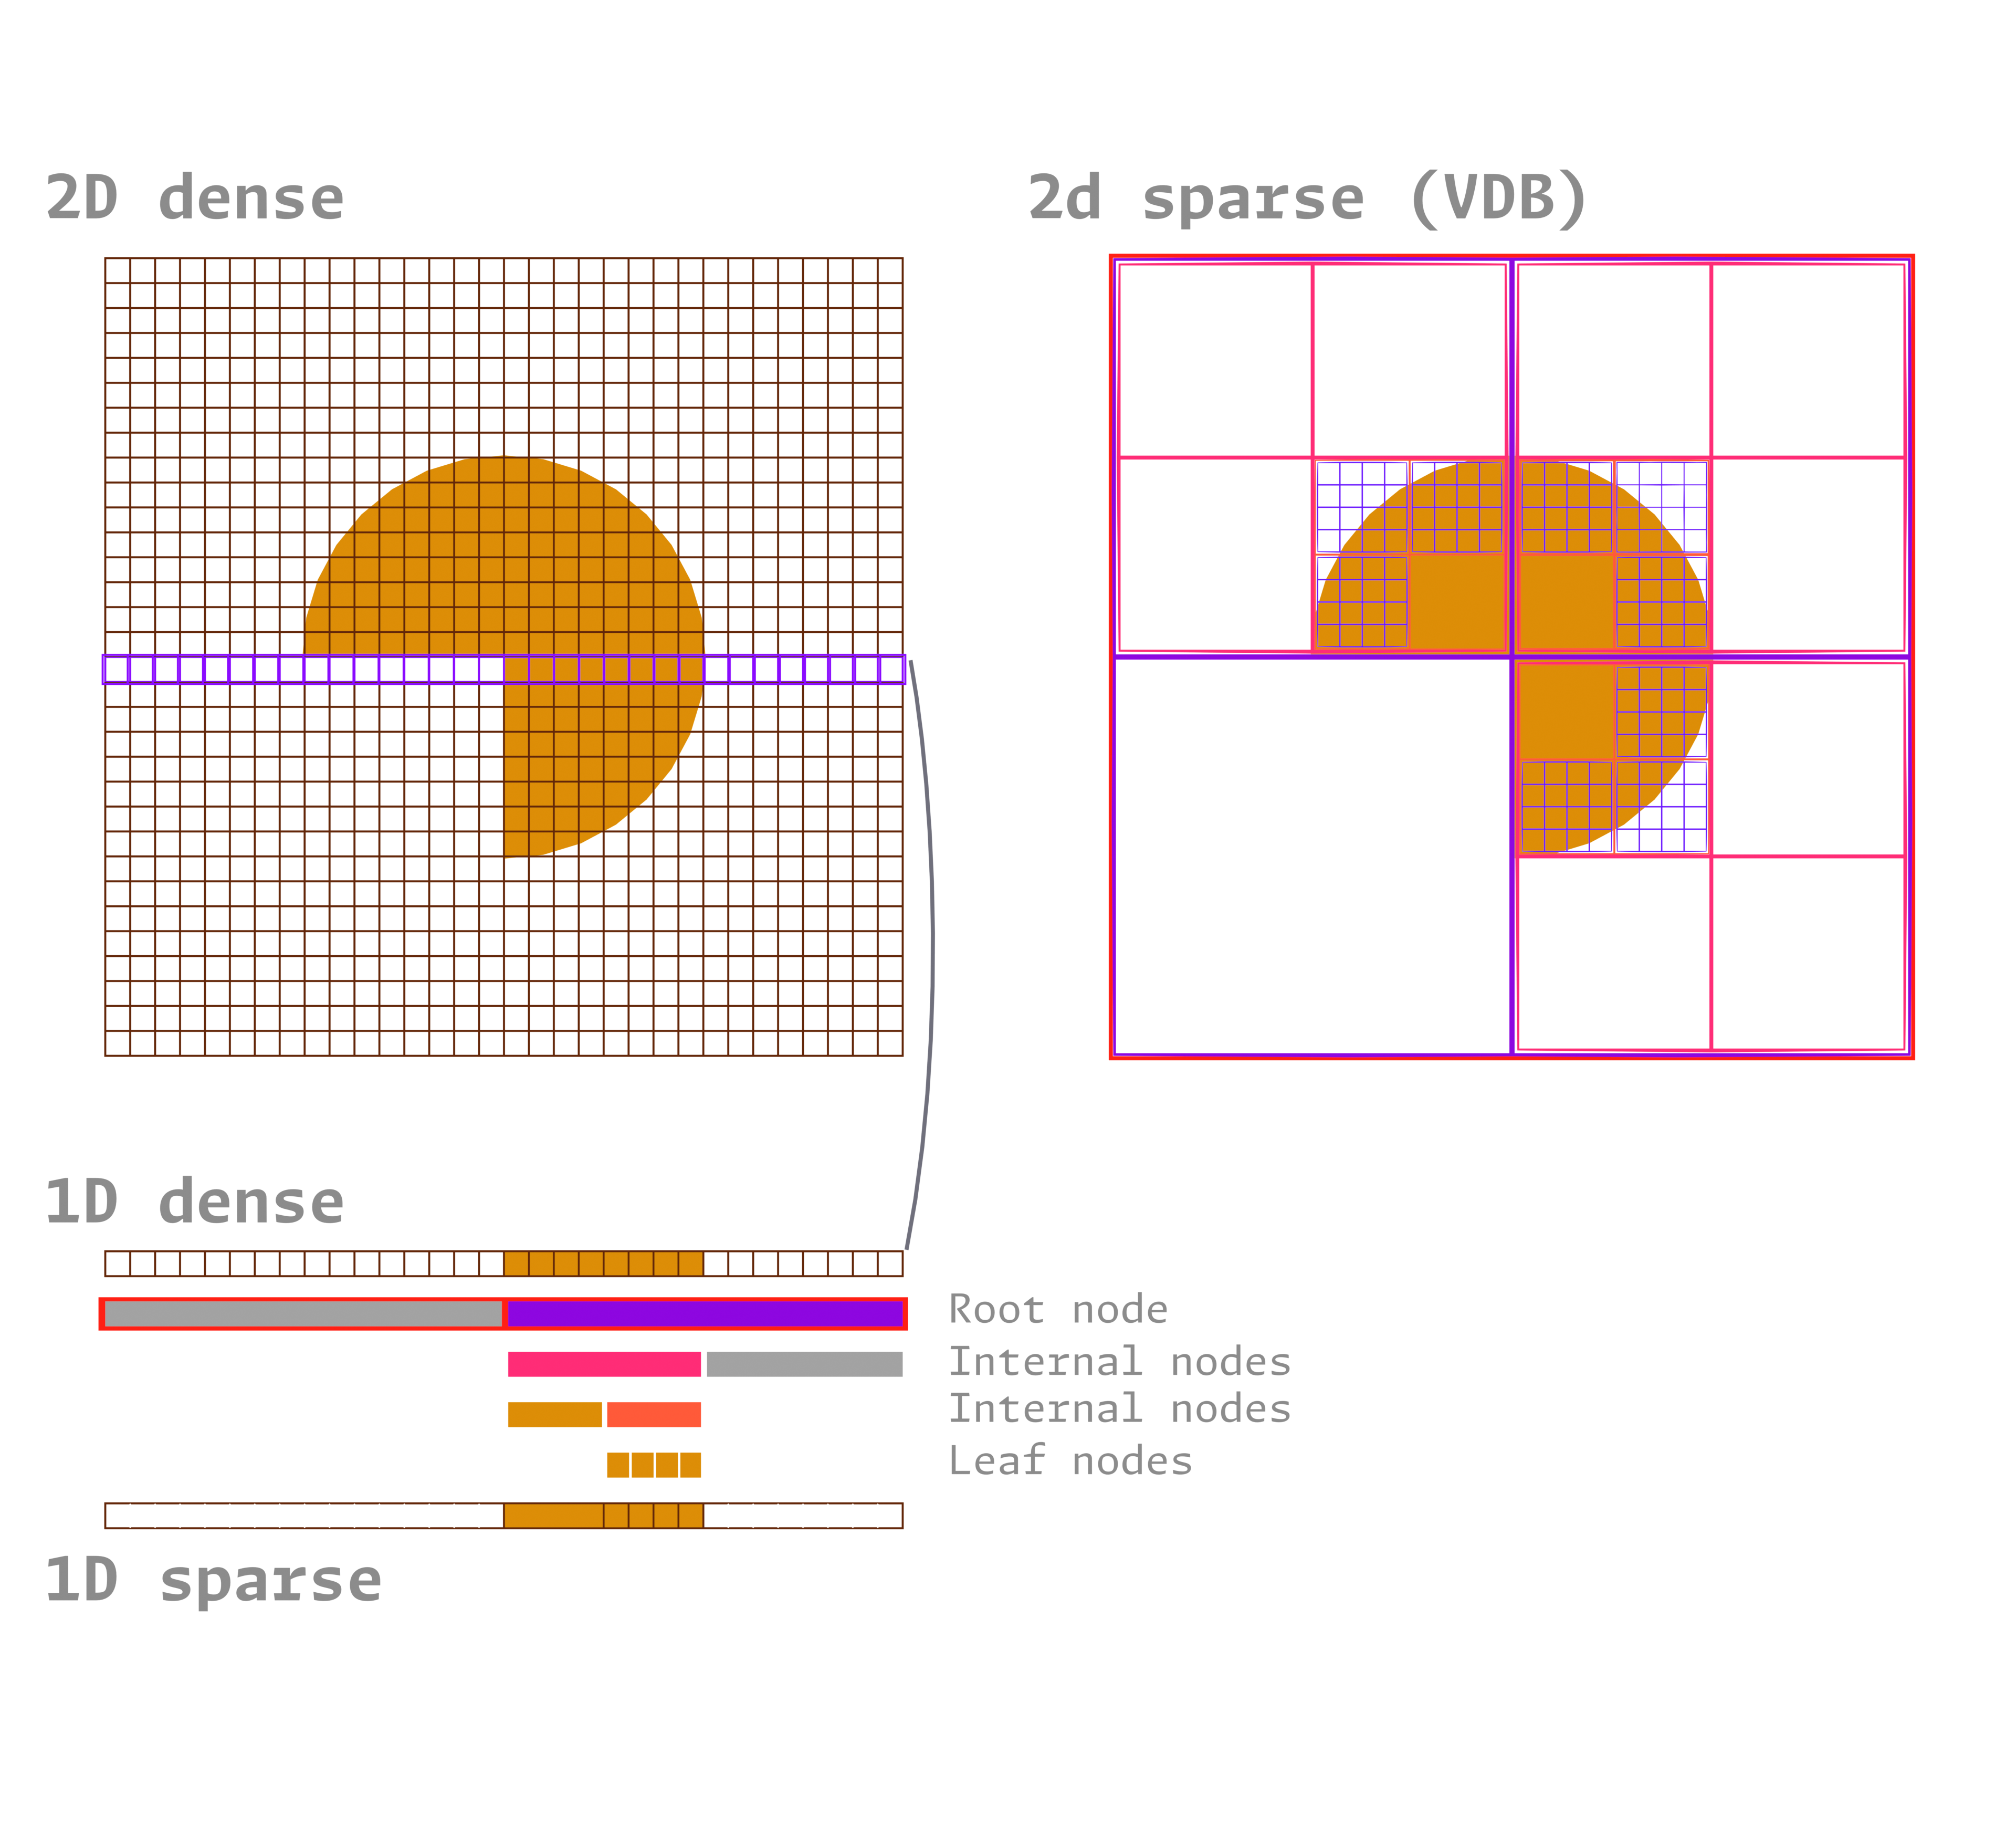
\includegraphics[width=\linewidth]{vdb}
  \caption{2D \& 1D slices of the VDB data structure representing three-quarters of a circle. Top left: 2D dense representation of the circle. Top right: 2D sparse representation of the VDB. Bottom left: Sparse representation of the 1D vdb. Usually, VDB nodes have many more child nodes, which would make it harder to visualise; hence, a smaller version of VDB is shown. This figure is an augmented version of the one in the original paper\supercite{vdb2013}}
\end{figure}

At the heart of the data structure are its three types of nodes: internal root and leaf. The VDB data structure is inherently general; each of the nodes' sizes can be modified depending on the application. However, in practice, only one specialisation of the VDB structure is used: the VDB543. This choice was made because the authors of the original paper\supercite{vdb2013} analysed a suite of possible shapes and sizes, and this configuration of VDB is the most balanced between performance and memory footprint for most practical applications.

\paragraph{Leaf Nodes} They are the lowest level in the tree structure. They store a 3D cubed grid of side length $2^{\log_{2} D}$ (i.e. only powers of 2). A leaf value in the grid can be a voxel's data, other associated data for empty values (such as SDF information), or an empty value.
Leaf nodes also store a value mask, a bit array meant to compactly determine whether a value at a specific coordinate in the 3D grid is voxel data or empty.

In the implementation, the trait \verb|Node| is defined, which gives some associated data and methods that leaf and internal nodes have.

\begin{lstlisting}[language=rust,caption={\texttt{Node} trait definition},captionpos=b,label={code:node}]
pub trait Node {
    /// LOG2_D of side length
    /// LOG2_D = 3 => `512 = 8 * 8 * 8` values
    const LOG2_D: u64;
    /// Total conceptual LOG2_D node
    const TOTAL_LOG2_D: u64;
    /// Total conceptual LOG2_D of child node
    const CHILD_TOTAL_LOG2_D: u64 = Self::TOTAL_LOG2_D - Self::LOG2_D;
    /// Side length
    const DIM: u64 = 1 << Self::LOG2_D;
    /// Total conceptual dimension
    const TOTAL_DIM: u64 = 1 << Self::TOTAL_LOG2_D;
    /// Size of this node (i.e. length of data array)
    const SIZE: usize = 1 << (Self::LOG2_D * 3);
    /// Total conceptual size of node, including child size
    const TOTAL_SIZE: u64 = 1 << (Self::TOTAL_LOG2_D * 3);
}
\end{lstlisting}

In \cref{code:node}, \verb|TOTAL_LOG2_D| represents the $\log_{2}$ of the total dimension of the node, meaning how much actual space the node occupies. Leaf nodes are at the bottom of the tree and do not have children, so this is the same as $\log_{2} D$, but this value will be relevant for internal nodes. All other attributes are determined at compile-time depending on the size of the node $\log_{2} D$.

\begin{quote}
  \paragraph{Sidenote on Coordinate Systems}

  It is very convenient for side lengths to be powers of two because of the way integers are stored in memory as binary values. To get the global coordinate of a node with \verb|TOTAL_LOG2_D| $= 3$ containing a point in global coordinates, the three least significant bits of each coordinate must be masked out. This operation can be done in a single CPU instruction for each coordinate.

\begin{lstlisting}[language=rust]
/// Give global origin of Node coordinates from `global` point
fn global_to_node(global: GlobalCoordinates) -> GlobalCoordinates {
    global.map(|c| (c >> Self::TOTAL_LOG2_D) << Self::TOTAL_LOG2_D)
}
\end{lstlisting}

Similarly, to get the relative coordinates of a global point within the node, are precisely the \texttt{TOTAL\_LOG2\_D} least significant bits.

\begin{lstlisting}[language=rust]
/// Give local coordinates relative to the Node containing `global` position
fn global_to_relative(global: GlobalCoordinates) -> LocalCoordinates {
    global.map(|c| (c & ((1 << Self::TOTAL_LOG2_D) - 1)))
}
\end{lstlisting}

This pattern of a few bit-wise operations can achieve any conversion between coordinate systems one might need, and all of these through operations are extremely fast to compute on modern CPUs.
\end{quote}

\Cref{code:leaf} shows a simplified definition of the leaf node data structure in the implementation. It has two fields: data, an array representing the 3D cube grid of values, and a value mask, a bit-mask carrying information on what each value represents, a voxel or empty space. the data array has has $2^{3\log_{2} D}$ entries(e.g. for $\log_{2} D = 3 \Rightarrow D = 8$ the leaf node has $8\times8\times8 = 512 = 2^{9}$ values). The value mask has the same number of bit entries but is stored as an array of unsigned 64-bit integers. Hence there are $\frac{D^{3}}{64}$ of them.

\begin{lstlisting}[language=rust, captionpos=b, caption={
    \texttt{LeafNode} definition.
    In the original paper\supercite{vdb2013}, node data is set as a union instead of an enum in order to save on memory space, only using the masks to determine the type of a particular value.
    In this implementation, an enum is used strictly for \emph{ergonomics}, as the extra 1 byte of memory per value is generally not expensive on heap-allocated memory.
    The value mask will still be crucial for the GPU version of VDB, where effective memory management is more important, and shading languages do not have enum support.
    In the \texttt{Node} trait implementation, since these nodes are the bottom level in the hierarchy (meaning they have no children), their in-memory dimensions are the same as their world space dimensions.
  }, label={code:leaf}]
pub struct LeafNode<ValueType, const LOG2_D: u64>
{
    pub data: [LeafData<ValueType>; (1 << (LOG2_D * 3))],
    pub value_mask: [u64; ((1 << (LOG2_D * 3)) / 64)],
}

pub enum LeafData<ValueType> {
    Tile(usize),
    Value(ValueType),
}

impl<ValueType, const LOG2_D: u64> Node for LeafNode<ValueType, LOG2_D>
{
    const LOG2_D: u64 = LOG2_D;
    const TOTAL_LOG2_D: u64 = LOG2_D;
}
\end{lstlisting}

The implementation is general both in the type of value stored at the voxel level, \verb|ValueType|, and in the Node dimension, \verb|LOG2_D|. This is achieved using Rust's generic const expressions feature \supercite{rust:generic} that is only available on the nightly toolchain. These work in a way akin to C++ templates, allowing the definition of types of static sizes chosen by the data structure user resolved at compile time. This approach allows for customising tree breadth and depth at compile time with no run-time overhead.

\paragraph{Internal Nodes} They sit between the root node and the leaf nodes, forming the middle layer of the tree structure.
They also store a 3D cubed grid of side length $2^{D}$ of values. An internal value can either be a pointer to a child node (leaf or internal) or a tile value, which is a value that is the same for the whole space that a child node in that position would cover.
Internal nodes also store a value mask and a child mask. These determine whether a value at a specific coordinate in the 3D grid is a child pointer, value type, or empty value.


\begin{lstlisting}[language=rust, captionpos=b, caption={
    \texttt{InternalNode} definition. Internal nodes have an extra field, the child mask, which is the same size as the value mask.
    Additionally, the internal data enum now has variants for a child pointer or 4 bytes of memory.
}]
pub struct InternalNode<ValueType, ChildType: Node, const LOG2_D: u64>
{
    pub data: [InternalData<ChildType>; (1 << (LOG2_D * 3))],
    pub value_mask: [u64; ((1 << (LOG2_D * 3)) / 64)],
    pub child_mask: [u64; ((1 << (LOG2_D * 3)) / 64)],
}

pub enum InternalData<ChildType> {
    Node(Box<ChildType>),
    Tile(u32),
}

impl<ValueType, ChildType: Node, const LOG2_D: u64> Node
    for InternalNode<ValueType, ChildType, LOG2_D>
{
    const LOG2_D: u64 = LOG2_D;
    const TOTAL_LOG2_D: u64 = LOG2_D + ChildType::TOTAL_LOG2_D;
}
\end{lstlisting}

When implementing the \verb|Node| the \verb|TOTAL_LOG2_D| is calculated by adding this node $\log_{2}D$ with the child node's total $\log_{2}D$.
For example, for an internal node with $log_{2}D = 4$ with children that are leaf nodes of $log_{2}D' = 3$, the internal node's $\log_{2}D_{{total}}$ will be $7$. This means that the internal node has $16\times16\times16$  children that each has $8\times8\times8$ voxels; the total number of voxels one of these internal nodes is $128\times128\times128$ or $2^{7}\times2^{7}\times2^{7}$.

It is important to note that all children of an internal node must be of the same type, which means each level in the tree only has one type of node. This ensures consistency in the coordinate system discussed previously.

\paragraph{Root Node} The root node is a single node at the top of the VDB hierarchy. Unlike typical nodes in a tree data structure, the root node in a VDB does not store data directly but instead serves as an entry point to the tree.
It contains a hash map indexed by global coordinates, linking to all its child nodes. This setup allows for quick access and updates, as the root node acts as a guide to more detailed data stored deeper in the hierarchy. Because its children nodes are stored by a hash map, it only stores information about space that has information to be stored(unlike an octree, where empty top-level nodes are frequent). The root node's primary role is to organise and provide access to internal nodes.


\begin{lstlisting}[language=rust, captionpos=b, caption={
    \texttt{RootNode} definition. \texttt{RootData} is either a pointer to a child or 4 bytes of data for a tile value.
  },label={code:root}]
pub struct RootNode<ValueType, ChildType: Node>
{
    pub map: HashMap<GlobalCoordinates, RootData<ChildType>>,
}

pub enum RootData<ChildType> {
    Node(Box<ChildType>),
    Tile(u32),
}
\end{lstlisting}

Finally, a VDB consists of a root node and some metadata associated with the volume, stored in the \verb|grid_descriptor| field. This metadata is generally only important when reading and writing \verb|.vdb| files.

\begin{lstlisting}[language=rust, captionpos=b, caption={\texttt{VDB} definition}, label={vdb:def}]
pub struct VDB<ValueType, ChildType: Node>
{
    pub root: RootNode<ValueType, ChildType>,
    pub grid_descriptor: GridDescriptor,
}
\end{lstlisting}

\subsection{VDB543}
$\rm{VDB}543$ is the most widely used configuration of the VDB data structure because it balances performance and memory footprint for most applications.
\begin{sloppypar}
  To refer to different shapes of the VDB data structure, by convention, they are named as ${\rm{VDB}[a_{0},a_{1},\dots, a_{n}]}$, $n$ layers of internal nodes with $\log_{2}D_{i}=a_{i}$ followed by a layer of leaf nodes with $\log_{2}D_{n}=a_{n}$. $\rm{VDB}543$ therefore has a layer of leaf nodes with $\log_{2}D_{n3} = 3$ and two layers of internal nodes, one with $\log_{2}D_{n4} = 4$ and the other with $\log_{2}D_{n5} = 5$.
\end{sloppypar}

To implement this type of VDB, a new type name for each type of node is created as shown in \cref{vdb543}, chaining them up the tree. This section will refer to these nodes as \texttt{Node3}s, \texttt{Node4}s and \texttt{Node5}s, respectively.

\begin{lstlisting}[language=rust, captionpos=b, caption={\texttt{VDB543} definition}, label={vdb543}]
pub type N3<ValueType> = LeafNode<ValueType, 3>;
pub type N4<ValueType> = InternalNode<ValueType, N3<ValueType>, 4>;
pub type N5<ValueType> = InternalNode<ValueType, N4<ValueType>, 5>;
pub type VDB543<ValueType> = VDB<ValueType, N5<ValueType>>;
\end{lstlisting}

To calculate how much the in-memory size, in bytes, of each node, the following calculation can be done by taking into account the size of the 3D grid together with the masks:
\begin{align*}
&\text{For leaf nodes:}& M &= D^{3} (v + 1) + \frac{D^{3}}{8} \\
&\text{For internal nodes (2 masks):}& M &= D^{3} (v + 1) + 2\frac{D^{3}}{8} \\
&\text{Where:}& D &= \text{dimension of node (side-length)} \\
&& v &= \text{number bytes the value type occupies (min. of 4)}
\intertext{Simillarly to find out how many voxels each node covers in world space:}
  &\textbf{Node3:}& D &= 2^3 = 8 \\
  && S &= D^3 = 8\times8\times8 = 512 \\
  &\textbf{Node4:}& D &= 2^4 = 16 \\
  && D_{t} &= 2^{4+3} = 128 \\
  && S &= D_{t}^3 = 128\times128\times128 = 2,097,152 \\
  &\textbf{Node5:}& D &= 2^5 = 32 \\
  && D_{t} &= 2^{5+4+3} = 4096 \\
  && S &= D_{t}^3 = 4096\times4096\times4096 = 68,719,476,736
\end{align*}

A single Node5 represents $4069^3$ voxels in space, just under $69$ billion.
Here, the power of the VDB data structure can be seen; models can have multiple \verb|Node5|s covering trillions of voxels in total, all of which can be accessed in $O(1)$ time by going three layers down the tree.


\subsection{Reading \texttt{.vdb files}}
VDB was introduced along with an associated file format \verb|.vdb|, which gives a compact data structure representation.
This section covers the part of the implementation that reads VDB files and stores them in memory.

Unfortunately, no official documentation of the format used to encode \verb| exists.vdb| files.
The only ``official'' resource available is the OpenVDB codebase\supercite{openvdb:doc}.
This article\supercite{vdbfile} reviews a file format reversed engineered from the OpenVDB codebase and the bytecode of \verb|.vdb| files.
The implementation uses this latter, reversed engineered format, which only supports \verb|.vdb| from version 218 onwards.

The following is an overview of the contents of a \verb|.vdb| file, as described in \cite{vdbfile}.

\newacronym{uuid}{UUID}{Universally Unique Identifier}

\begin{enumerate}
  \item Header
        \begin{enumerate}
          \item Magic number spelling out `` BDV'' (8 bytes)
          \item File version (u32)
          \item Library major and minor versions (2 u32s)
          \item Grid offsets to follow flag (u8)
          \item \acrshort{uuid} (128-bit)
          \item Metadata entries, length-based list
          \item Number of grids (u32)
        \end{enumerate}
        Since multiple grids can be stored in a single file, the following steps are repeated for all grids.
  \item VDB Grid
        Grids are composed of a grid metadata and a tree. In the engine's implementation, they are just called \verb|VDB|, as seen in \cref{vdb:def}.
        \begin{enumerate}
          \item Name of the grid (length-based string)
          \item Grid type (length-based string) \\
                e.g. \verb|Tree_float_5_4_3| refers to a VDB543\<f32\> in the implementation.
                This type $T$ will determine the data size when reading the tree data later on.
          \item Instance parent (u32)
          \item Byte offset to grid descriptor (u64)
          \item Start and end location of grid data (2 u64)
          \item Compression flags (u32)
          \item\label{file:meta} Grid metadata, length-based list of metadata entries \\
                An entry consists of an entry name as a length-based string, an entry type as a length-based list, and actual data
          \item Transform matrices to apply to voxels coordinates to convert from index space to world space (4x4 f64s )
        \end{enumerate}
  \item VDB Tree
        \verb|.vdb| files can have multiple trees associated with the grid; hence, this step can be repeated for all trees in a grid.
        \begin{enumerate}
          \item the number 1 (u32)
          \item background value of root node ($T$)
          \item Number of tile values in root node (u32)
          \item Number of children of the root node (u32)
          \item Descend the tree depth-first describing its \emph{topology}.
                For each internal node, starting from the top layer.
                The idea is to first describe the tree topology and the nodes' hierarchy, then in a second pass in \cref{file:rec1} to give the actual voxel data.
                \begin{enumerate}
                \label{file:rec}
                  \item The origin of the node, only for top-level nodes (three i32)
                  \item The child mask, only for internal nodes ($D^3$ bits)
                  \item The value mask ($D^3$ bits)
                  \item Compression flags
                  \item Values, only for internal nodes ($D^{3} \times T$)
                  \item Repeat \cref{file:rec} for every child in order of the mask
                \end{enumerate}
          \item\label{file:rec1} Leaf Node data as value mask + values ($D^{3}$ bits + $D^{3}\timesT$)

                The LeafNodes are given in the same order they were covered in \cref{file:rec}
        \end{enumerate}
\end{enumerate}

In the implementation of VDB file handling within the rendering engine, a specialised streaming reader, termed \texttt{VdbReader}, is designed to manage the reading process efficiently.
This approach optimises memory usage by incrementally processing the file's content rather than loading the entire file into memory simultaneously.
This method is particularly beneficial since VDB files can have hundreds of megabytes.

The \texttt{VdbReader} is structured to sequentially process sections of the VDB file, creating nodes as it reads and assembles them into the complete VDB data structure shown in \cref{vdb:ds}.

\texttt{VdbReader} reads from the VDB file according to the grid descriptors, constructing nodes from the data, ensuring each node is placed within the VDB hierarchy. This process involves interpreting the file's byte stream according to the VDB format specifications and converting this data into a usable form within the rendering engine.

\begin{lstlisting}[language=rust, captionpos=b, caption={
    \texttt{VdbReader} definition: \texttt{reader} is file stream handler, \texttt{grid\_descriptors} hold the metadata given in \cref{file:meta}.
    \texttt{VdbReader} implementation: The method \texttt{read\_vdb\_grid} is shown, which is called after the file header is handled, and returns a VDB if the file contents match the expectations from the header; if not, it returns an error.
  }, label={vdb:read}]
pub struct VdbReader<R: Read + Seek> {
  reader: R,
  pub grid_descriptors: HashMap<String, GridDescriptor>,
}

impl<R: Read + Seek> VdbReader<R> {
  ...
  pub fn read_vdb_grid<T: VdbValueType>(&mut self, name: &str) -> Result<VDB<T>> {
    let grid_descriptor = self.grid_descriptors.get(name).cloned()
    .ok_or_else(|| ErrorKind::InvalidGridName(name.to_owned()))?;
    grid_descriptor.seek_to_grid(&mut self.reader)?;

    if self.header.file_version >= OPENVDB_FILE_VERSION_NODE_MASK_COMPRESSION {
      let _: Compression = self.reader.read_u32::<LittleEndian>()?.try_into()?;
    }
    let _ = Self::read_metadata(&mut self.reader)?;

    let mut vdb = self.read_tree_topology::<T>(&grid_descriptor)?;
    self.read_tree_data::<T>(&grid_descriptor, &mut vdb)?;

    Ok(vdb)
  }
}
\end{lstlisting}

With this reader implemented any \texttt{.vdb} file can be brought into the rendering engine, which will provide a series of models from the internet to use during testing and in the results section. Additionally, thanks to the widespread adoption of VDB in modern 3D modelling tools like Blender and Maya, any 3D model can be converted to VDB, essentially enabling any mesh to be pulled into the engine, albeit by stepping out of the engine first.

\subsection{GPU VDB}
\newacronym{cuda}{CUDA}{Compute Unified Device Architecture}

The next step is designing a version of VDB that can be passed to the GPU in compute shaders. The authors of OpenVDB created a version of the VDB data structure, NanoVDB\supercite{nanovdb:doc}, that can use \acrshort{cuda} instructions for GPU acceleration on the data structure. NanoVDB is explained very well by the authors in this article on the Nvidia blog \cite{nanovdb:art}.

At this point, this implementation diverges from the OpenVDB library. This project aims to optimise performance while supporting as many platforms as possible, and CUDA instructions are only supported on Nvidia hardware.

This section presents a custom implementation for a GPU-compatible, read-only version of VDB543. This version splits VDBs into two separate components:

\textbf{(a) Mask group} This is a collection of five bindings, each an array of u32s that stores the masks for all nodes: two mask arrays for each internal node layer (Node5 and Node4) and one mask array for the leaf layer (Node3). Each array has length $N\frac{D^{3}}{32}$, where $N$ is the number of nodes it refers to. These five buffers are passed to the GPU in a storage buffer group, each in a separate binding.

\begin{lstlisting}[language=rust, captionpos=b, caption={
    \texttt{MaskUniform} definition: Each type of mask list is a separate binding. An additional binding is created to store the origins of the top-level Node5 nodes.
    \texttt{MaskUniform} implementation: The \texttt{bind} method generates all data needed to pass the mask group to compute shaders. The \texttt{create\_bind\_group\_layout}
    function is the critical part of this process; each binding is a storage buffer type with read-only access.
}]
pub struct MaskUniform {
  kids5: Vec<Node5Mask>,
  vals5: Vec<Node5Mask>,
  kids4: Vec<Node4Mask>,
  vals4: Vec<Node4Mask>,
  vals3: Vec<Node3Mask>,
  origins: Vec<[i32; 4]>,
}

impl MaskUniform {
  pub fn bind(&self, device: &Device) ->
  ([Buffer; 6], [Vec<u8>; 6], BindGroup, BindGroupLayout) {
    let buffer_contents = self.get_contents();
    let buffers = self.create_buffers(device, &buffer_contents);
    let layout = self.create_bind_group_layout(device);
    let bind_group = self.create_bind_group(&buffers, &layout, device);

    (buffers, buffer_contents, bind_group, layout)
  }
  ...
  fn create_bind_group_layout(&self, device: &Device) -> BindGroupLayout {
    let entries = &(0..=5)
    .map(|binding| wgpu::BindGroupLayoutEntry {
      binding,
      visibility: wgpu::ShaderStages::COMPUTE,
      ty: wgpu::BindingType::Buffer {
        ty: wgpu::BufferBindingType::Storage { read_only: true },
        has_dynamic_offset: false,
        min_binding_size: None,
      },
      count: None,
    })
    .collect::<Vec<_>>()[..];

    device.create_bind_group_layout(&wgpu::BindGroupLayoutDescriptor {
      entries,
      label: Some("Mask Bind Group Layout"),
    })
  }
}
\end{lstlisting}

    With the bind group created and integrated into the pipeline, compute shaders can now access the topology of the data.

\begin{lstlisting}[language=rust, captionpos=b, caption={
    wgsl version of the mask arrays. Each buffer is divided into parts based on the size of the node it tackles. This enables getting all the masks of a node with a particular index by simply indexing them into the mask array. For example, \texttt{kids5[0]} would give the first child mask for the Node5 at index 0.
}]
struct Node5Mask { m: array<u32, 1024>, }; // 32^3/32
struct Node4Mask { m: array<u32, 128>, };  // 16^3/32
struct Node3Mask { m: array<u32, 16>, };   // 8^3/32

@group(3) @binding(0)
var<storage, read> kids5: array<Node5Mask>;
@group(3) @binding(1)
var<storage, read> vals5: array<Node5Mask>;
@group(3) @binding(2)
var<storage, read> kids4: array<Node4Mask>;
@group(3) @binding(3)
var<storage, read> vals4: array<Node4Mask>;
@group(3) @binding(4)
var<storage, read> vals3: array<Node3Mask>;
@group(3) @binding(5)
var<storage, read> origins: array<vec3<i32>>;
\end{lstlisting}
    A key part of this representation is the order in which node masks are given in each particular binding, meaning how the node index in the value mask is related to that same node in the CPU-based data structure. The approach is the same as when reading \texttt{.vdb} files: a depth-first descent of the tree topology. The order of nodes in the GPU VDB representation is the same as the order in which they appear in the file.


\textbf{(b) Atlas group} This bind group stores all the voxel and child ``pointer'' packed into atlases as 3D textures. This data type is the perfect storage type for 3D grids because it enables retaining relative coordinates within the nodes while packing them next to each other in memory. This technique was inspired by two articles \cite{octree:1,octree:2}. The latter presents a packing termed $N^{3}$-tree, which presents a method to serialise octree nodes in an array of textures and store indices in that same array to represent children's nodes. This idea is not directly applicable to VDB since nodes at different depths have different sizes, so much of the space would be wasted since most nodes are smaller than the top-level Node5 nodes. However, this idea can be expanded by using a different texture atlas for every type of node and cross-referencing between each layer. For VDB543, This entails having three different atlases, with the values of the first two (corresponding to Node5s and Node4s) indexing into the Node4 and Node3 atlases, respectively.

\begin{lstlisting}[language=rust, captionpos=b, caption={
    \texttt{NodeAtlas} definition: The three fields are the sizes of each atlas.
    The \texttt{create\_textures} creates three textures, sets the correct dimensions and sets value type to \texttt{R32Uint} represent a 4-byte single channel, which can be used depending on what the value represents.
    The \texttt{create\_bind\_group\_layout} prepare the binding for compute shaders, setting the sample type to \texttt{Uint} to ease access to the atlases' data.
},label={atlas2idx}]
pub struct NodeAtlas {
  size5: [u32; 3],
  size4: [u32; 3],
  size3: [u32; 3],
}

impl NodeAtlas {
  pub fn bind(&self, device: &Device)
  -> ([Texture; 3], BindGroup, BindGroupLayout) {
    let textures = self.create_textures(device);
    let views = textures.iter()
      .map(|texture| self.create_texture_view(&texture))
      .collect::<Vec<_>>().try_into().unwrap();
    let bind_group_layout = self.create_bind_group_layout(device);
    let bind_group = self.create_bind_group(device, &bind_group_layout, &views);

    (textures, bind_group, bind_group_layout)
  }

  fn create_textures(&self, device: &Device) -> [Texture; 3] {
    [self.size5, self.size4, self.size3].map(|[w, h, d]| {
      device.create_texture(&wgpu::TextureDescriptor {
        size: wgpu::Extent3d {
          width: w,
          height: h,
          depth_or_array_layers: d,
        },
        mip_level_count: 1,
        sample_count: 1,
        dimension: wgpu::TextureDimension::D3,
        format: wgpu::TextureFormat::R32Uint,
        usage: wgpu::TextureUsages::TEXTURE_BINDING | wgpu::TextureUsages::COPY_DST,
        label: Some("Atlas Texture"),
        view_formats: &[],
      })
    })
  }
  ...

  fn create_bind_group_layout(&self, device: &Device) -> BindGroupLayout {
    device.create_bind_group_layout(&wgpu::BindGroupLayoutDescriptor {
      label: Some("Atlas Texture Bind Group Layout"),
      entries: &[0, 1, 2].map(|binding| wgpu::BindGroupLayoutEntry {
        binding,
        visibility: wgpu::ShaderStages::COMPUTE,
        ty: wgpu::BindingType::Texture {
          sample_type: wgpu::TextureSampleType::Uint,
          view_dimension: wgpu::TextureViewDimension::D3,
          multisampled: false,
        },
        count: None,
      }),
    })
  }
}
\end{lstlisting}
        With the bindings implemented, fetching these in the shader code is possible, finally bringing VDB data to the GPU.

\begin{lstlisting}[language=rust, captionpos=b, caption={
            wgsl atlas bindings, to get a value in the atlas at point $(x,y,z)$, \texttt{textureLoad(x,y,z).r} is called since all the data is stored on the red channel
},label={atlas2idx}]
@group(2) @binding(0)
var node5s: texture_3d<u32>;
@group(2) @binding(1)
var node4s: texture_3d<u32>;
@group(2) @binding(2)
var node3s: texture_3d<u32>;
\end{lstlisting}

  Since these are 3D textures, a way of converting the indexing in the mask buffers to these texture atlases is needed. Atlases are cube-shaped, and nodes are packed in them by stacking them next to one another with coordinate priority $x > y > z$ in the same depth-first order as discussed previously. This idea yields a straightforward transformation between the indexes of the mask buffers and the coordinates in the texture atlas, shown in \cref{atlas2idx}

\begin{lstlisting}[language=rust, captionpos=b, caption={wgsl transformation from index of node to coordinate in atlas},label={atlas2idx}]
fn atlas_origin_from_idx(idx: u32, dim: u32) -> vec3<u32> {
  return vec3(idx \% dim, (idx / dim) \% dim, idx / (dim * dim));
}
\end{lstlisting}

The two types of VDB were covered: GPU and CPU-based. To convert from the CPU-based structure to the GPU-based structure one simply recursively descends the tree in deaoth-first order, adding nodes to their corresponding atlases one by one, stacking them in the 3D texture.
\end{enumerate}

\subsection{SDF for VDB}\label{vdb:sdf}
This section outlines what distance field data is injected into empty VDB tiles and how this information can be computed from a normal VDB.

In a standard grid, \acrshort{sdf}s encode the Manhattan or Chebyshev distance\supercite{chebyshev} to the nearest voxel.
Splitting up the SDF calculation at each level of the hierarchy can extend this to hierarchical grids.
Empty nodes on the higher level of the hierarchy will store the nearest distance to another node that is not empty (meaning it is either a tile value or it is subdivided into children).

\textbf{Computing the SDF}

A generalised (3D) version of the Chamfer Distance Transform algorithm\supercite{chamfer} is used to calculate the distance field information.
It is essentially a two-pass method.
\begin{enumerate}
  \item \emph{Forward Pass:} Starting from the top-left corner of the grid, this pass iterates through each cell. It calculates the minimum distance to the nearest feature by considering the already processed neighbours (typically the cells immediately above and to the left of the current cell). Each cell updates the distance by comparing its current value with the already computed values from these neighbours, typically using predefined weights for horizontal/vertical and diagonal steps.

  \item \emph{Backward Pass:} Beginning from the bottom-right corner, this pass iterates back through the grid. It now considers the cells that were not accessible in the forward pass (typically the cells immediately below and to the right of the current cell). Again, it updates the distances in each cell by considering the shortest computed distances from these neighbours.
\end{enumerate}
This algorithm has a straightforward 3D generalisation, starting at the top-left-near corner in the first pass and the bottom-right-far corner in the second pass.

This algorithm can be optimised by considering that for hierarchical data structures, SDF data is virtually independent between levels of the hierarchy.
This level of independence allows the computation to be run on a separate thread for each layer in the hierarchy.

%%% Local Variables:
%%% mode: latex
%%% TeX-master: "../main"
%%% End:
